\chapter{Implementation of noise for timing in simulations.}
\label{appendix:noise}

Due to the nature of the detector triggering, noise can't be extracted like the previous CALICE physics prototypes with external triggers between between spills. Moreover if no validation signal is provided by the trigger scintillators, the chip removes noise events stored in memory.

One way to avoid this, one can use real events to extract noise. This is can be efficiently done with muon runs as a track in present in the calorimeter due to the muon. By removing the track and keeping remaining hits, noise can be extracted. Muon runs from 24647 to 24656 are used for noise extraction. The events are selected by the cuts shown in table \ref{table:noise_sel}.

\begin{table}[htb!]
	\centering
	\caption{Selection cuts for noise extraction from muon runs.}
	\label{table:noise_sel}
	\resizebox{0.9\textwidth}{!}{%
	\begin{tabular}{@{}p{4cm} p{3cm} p{6cm}@{}}
		\hline
		\multicolumn{1}{l}{\textbf{Name}} & \textbf{Beam Energy} & \textbf{Cut}\\
		\hline
		\multirow{3}{*}{Noise selection}& All & $n_{hits}$ in a tower > 7\\& All & 0 < $n_{hits}$ < 30\\& All & $n_{hits}$ in layer < 3\\
		\hline
	\end{tabular}
	}
\end{table}

Remaining hits after track removal are considered as noise hits. Initially, the time of these are in TDC values. To get an approximation of the noise distribution, the time of a noise hit is randomly shifted by a flat distribution between 500 and 3500 ns. This acts as a time reference for these hits and thus give a quite good description of the noise time distribution. The figures \ref{fig:noise_energy} and \ref{fig:noise_time} show the energy and time distribution of noise hits.

\begin{figure}[htbp!]
	\begin{subfigure}[t]{0.49\textwidth}
		\centering
		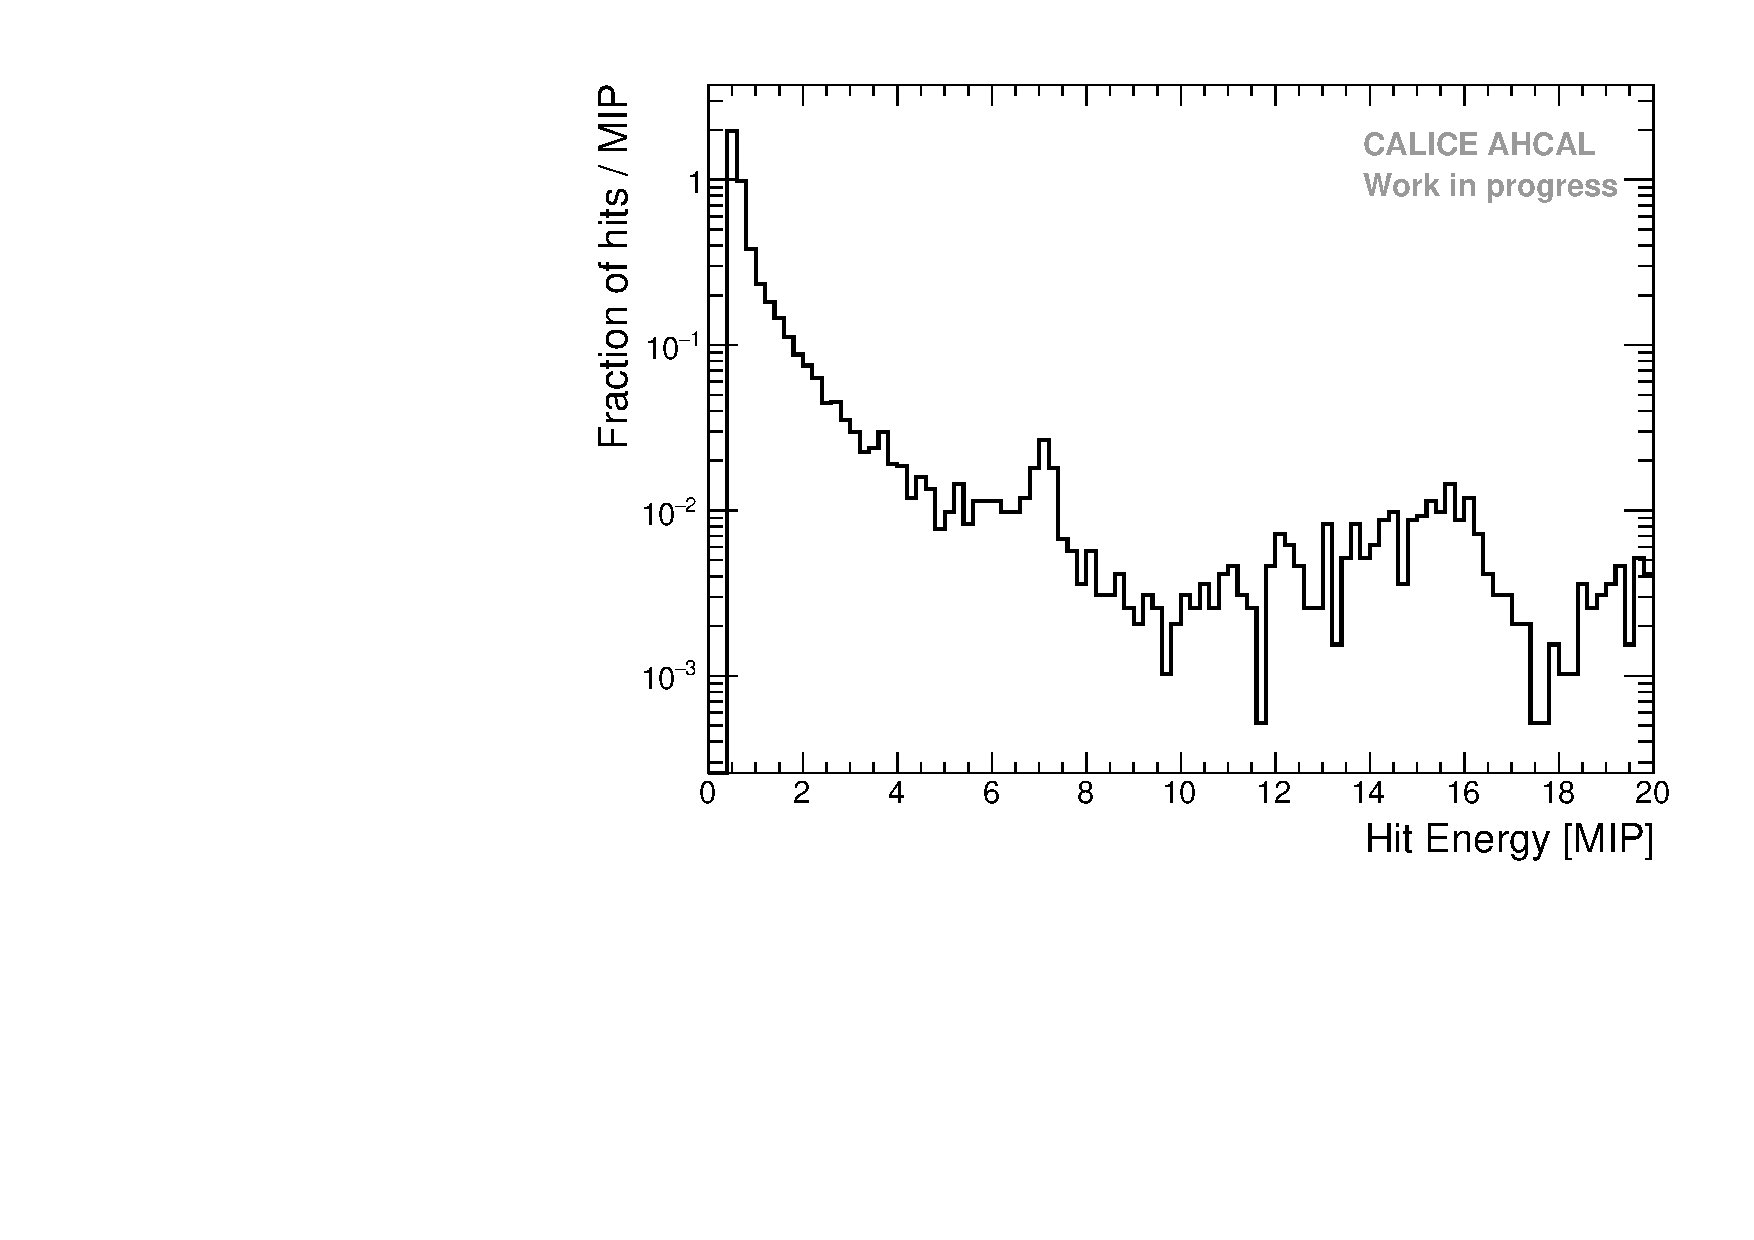
\includegraphics[width=1\linewidth]{../Thesis_Plots/Timing/Muons/Plots/Noise_Energy_Flat.pdf}
		\caption{Energy distribution of noise hits.} \label{fig:noise_energy}
	\end{subfigure}
	\hfill
	\begin{subfigure}[t]{0.49\textwidth}
		\centering
		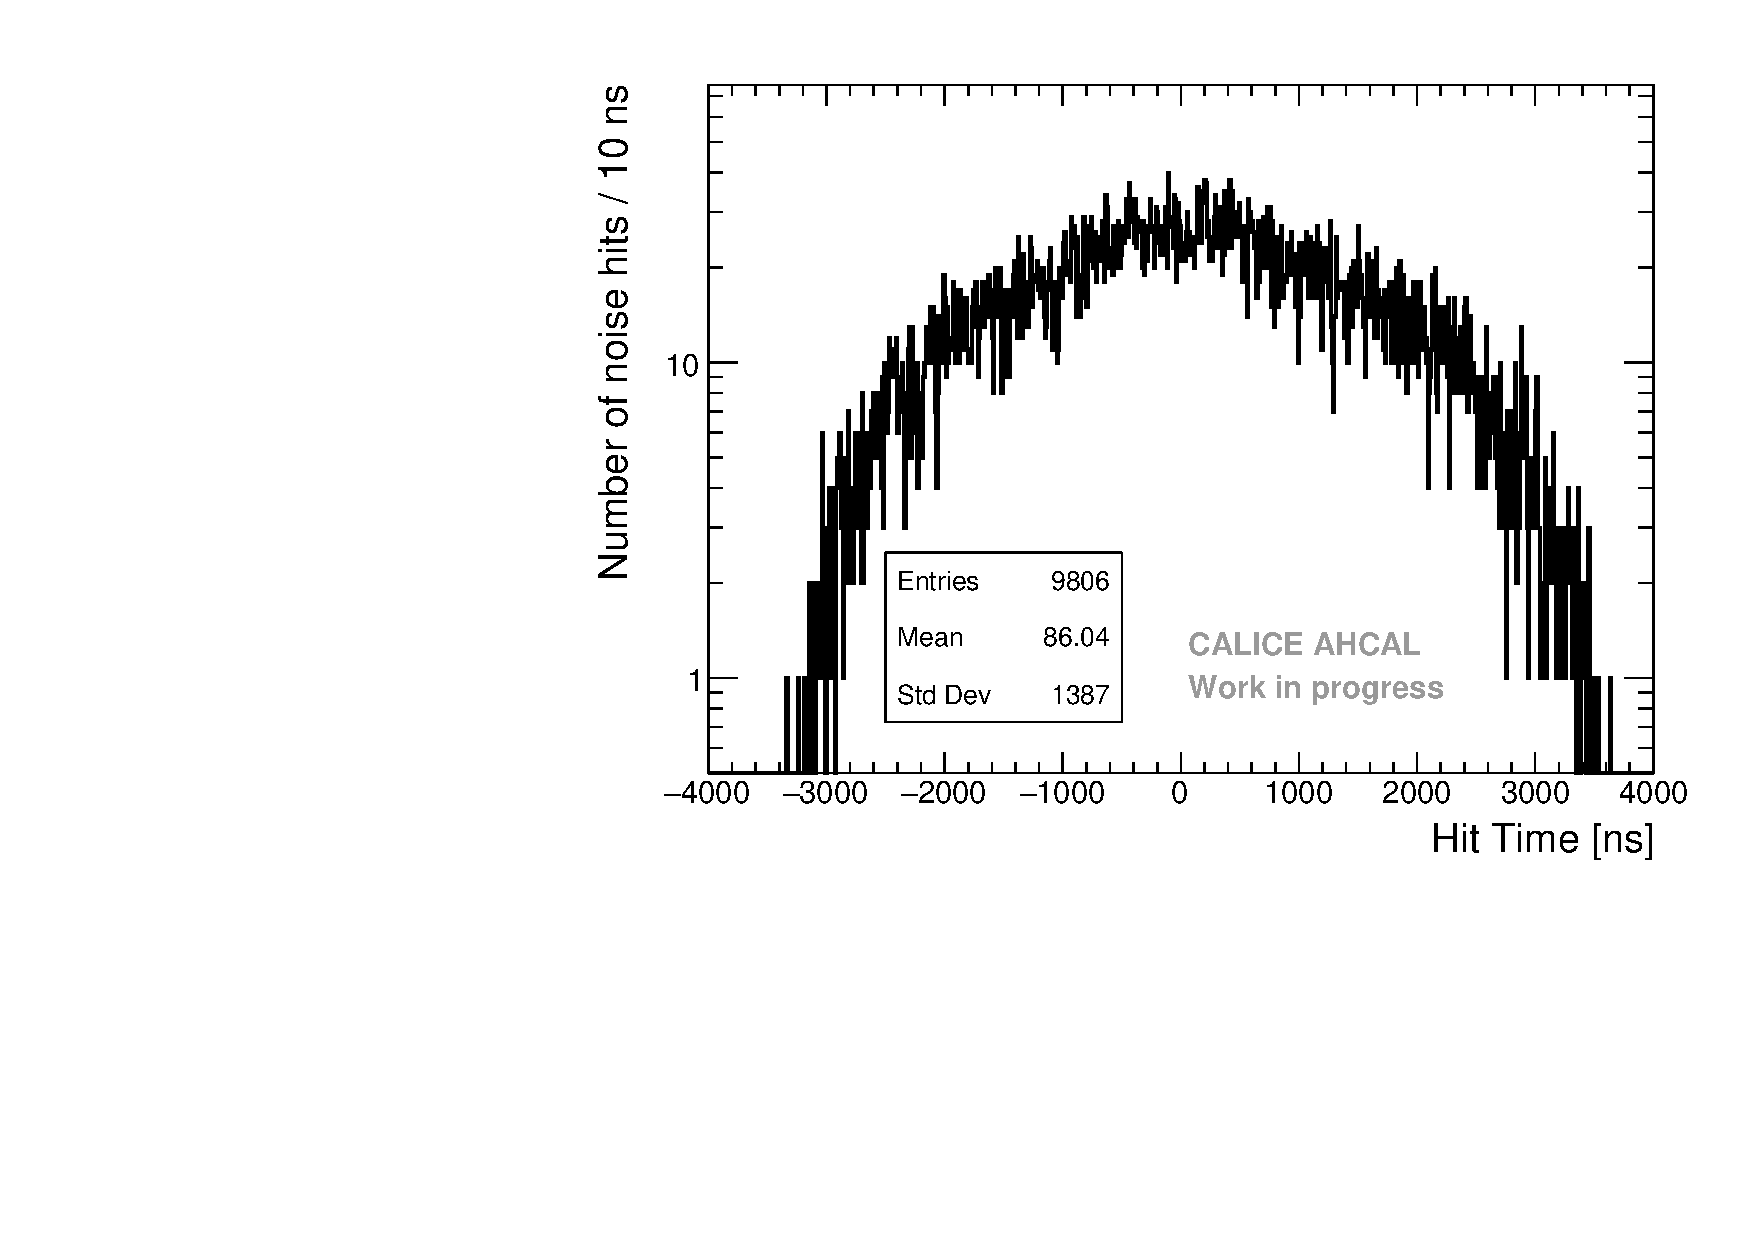
\includegraphics[width=1\linewidth]{../Thesis_Plots/Timing/Muons/Plots/Noise_Time_Flat.pdf}
		\caption{Time distribution of noise hits.} \label{fig:noise_time}
	\end{subfigure}
	\caption{\subref{fig:noise_energy}) Most of the fraction of noise hits have an energy under 2 MIPs. Higher hit energies may be due to delta electrons from muon tracks but is not expected to have a great impact on timing. \subref{fig:noise_time}) The shape of the time distribution of noise hits is very important to reproduce well the data in simulation.}
\end{figure}

The introduction of noise for timing is very important to compare data and simulation especially for pions where a late tail is present.
